\documentclass[english, biblatex]{lni}
\addbibresource{informatika.bib}
\usepackage{graphicx}
\usepackage{amsmath}
\graphicspath{ {./pictures/} }
%%% To write an article in English, please use the option ``english'' in order
%%% to get the correct hyphenation patterns and terms.
%%% \documentclass[english]{class}
%%
\begin{document}
%%% Mehrere Autoren werden durch \and voneinander getrennt.
%%% Die Fußnote enthält die Adresse sowie eine E-Mail-Adresse.
%%% Das optionale Argument (sofern angegeben) wird für die Kopfzeile verwendet.
\title[AI in Plant Breeding]{Integrating Big Data and Deep Learning for Improved Wheat (Triticum aestivum) Grain Yield Predictions}
%%%\subtitle{Untertitel / Subtitle} % if needed
\author[Abhishek Gogna \and Yusheng Zhao \and Jochen C. Reif]
{Abhishek Gogna\footnote{Leibniz Institute of Plant Genetics and Crop Plant Research (IPK), Department of breeding research, Correnstrasse 3, 06466, Gatersleben \email{gogna@ipk-gatersleben.de}} \and
Yusheng Zhao\footnote{Leibniz Institute of Plant Genetics and Crop Plant Research (IPK), Department of breeding research, Correnstrasse 3, 06466, Gatersleben \email{zhao@ipk-gatersleben.de}} \and
Jochen Reif\footnote{Leibniz Institute of Plant Genetics and Crop Plant Research (IPK), Department of breeding research, Correnstrasse 3, 06466, Gatersleben \email{reif@ipk-gatersleben.de}}}
\startpage{1} % Beginn der Seitenzählung für diesen Beitrag / Start page
\editor{Abhishek} % Names of Editors
\booktitle{Informatika} % Name of book title
\yearofpublication{2023}
%%%\lnidoi{18.18420/provided-by-editor-02} % if known
\maketitle
\begin{abstract}
Machine learning, particularly Deep learning methods are gaining spotlight within the plant breeding community, given the advantages these offer for modeling nonlinear interactions. The same is additionally fueled by the injection of data management principles into the field, ushering in an era of BigData in plant breeding. In addition to the traditional ones like genotypic and phenotypic data, diverse data sources have been identified and stored structurally to predict important traits across main crops like wheat and maize. However, the research into models that combine the utility of deep learning and information in BigData is still in its infancy within the community. Further developments in this area are crucial for a sustainable increase in model prediction accuracies. To address this issue, we curate a unique data resource of Wheat Big Data and benchmark different deep learning models against the community standard GBLUP and Extended-GBLUP models using different cross-validation regimes. The deep learning models perform at least comparable to the GBLUP and Extended-GBLUP models and hold potential for use in plant breeding, especially given the speed advantage realized with these models. In conclusion, it is proposed that developments in this direction will benefit from a better understanding of the role of deep learning model architecture, network types, and efficient methods of model deployment.
\end{abstract}
\begin{keywords}
E-GBLUP \and CNN %Keyword1 \and Keyword2
\end{keywords}
%%% Beginn des Artikeltexts
\section{Introduction}
Breeding programs benefit from the integration of genomic prediction into the selection process at various stages of the variety development cycle \cite{piepho_blup_2008}. Genomic selection allows for the identification of promising germplasm without the need for extensive field testing. However, in cases where trait heritabilities are low, such as with wheat grain yield during the later stages of development, this approach may not be feasible. Wheat grain yield is a complex phenotype influenced by multiple factors, including the crop growth environment, genotype, and genotype by environment (GxE) interactions \cite{cooper_extending_2023}. To improve grain yield predictions, it is crucial therefore to account for environment as well as GxE interaction effects, particularly when predicting the performance of tested or untested genotypes in environments outside the training population (TG-O-TPE, UG-O-TPE). Incorporating GxE effects has been shown to enhance the accuracy of grain yield predictions. However, due to the non-linear nature of these effects and the challenges associated with precise measurement, they are often approximated \cite{jarquin_reaction_2014} or disregarded, leading to potential inaccuracies in predictions \cite{crossa_genome_2022}.

BigData generated from curated, unbalanced datasets, corrected for design effects of individual environments, holds significant potential for improving prediction accuracies, particularly when GxE effects are not considered \cite{zhao2021unlocking}. However, limited research has been conducted thus far on the utilization of Big Data to capture GxE and predict TG-O-TPE and UG-O-TPE.

Fortunately, recent advancements in artificial intelligence, particularly in machine learning and deep learning, present a unique opportunity to leverage Big Data for learning non-linear interactions such as GxE. Among the various classes of deep learning models, convolutional neural networks (CNNs) have demonstrated robust performance in capturing nonlinear interactions between input features. They achieve this through multiple rounds of convolutions, extracting higher-level features from the underlying inputs. The present study integrates convolutional neural networks (CNNs), Big Data, and efficient approximation methods to predict grain yield in winter wheat while considering GxE effects. The study has two primary objectives:

\begin{itemize}
    \item Propose and discuss a framework to integrate genotypic, phenotypic and environment data for use in predicting wheat grain yield
    \item Develop and benchmark a CNN model against extended G-BLUP (EG-BLUP)
\end{itemize}

\section{Methods}

\textit{Phenotypic data corrected for experimental design as well as environment effect was analyzed}

The design effect-corrected phenotypic data for six experimental series was inherited from Zhao et al. \cite{zhao2021unlocking}, and an additional series was added to further complement the phenotypic data \cite{gogna_gabi_2022}. This curated data is denoted as BLUEs\textsubscript{wtn}. Correction for the environmental effect in the integrated phenotypic data was performed according to the following model:

\hspace{0.5cm}\begin{minipage}{\dimexpr\linewidth-0.5cm}
\begin{equation}
y = \mu + G\tau + Eu + e,
\end{equation}
\end{minipage}

where \(y\) is vector of the design effect corrected grain yield values, \(G\) is the design matrix of genotypes, \(E\) is the design matrix of environments, \(\tau\) is the vector of genotypic effects, \(u\) is the vector of environmental effects, and \(e\) is the vector of residuals.

For the derivation of means across locations (Best Linear Unbiased Estimates, abbreviated as BLUEs), \(\tau\) was assumed to be a fixed effect, whereas \(u\) was assumed to be a random effect. The respective variances of \(u\) and \(e\) were set to NIID (normally, independently, and identically distributed). The model was implemented in ASREML-4.2 inside R.

\textit{Haplotype based imputation was used to fill missing values in the integrated SNP array data}

Similar to the phenotypic data, the integrated genotypic data for six experimental series was inherit-ed from \cite{zhao2021unlocking} and additional genotypic data was added to supplement the phe-notypic data. In total this data holds the genetic information for approximately 14k genotypes spread across nine chips of varying marker densities and genotype overlap. The integrated genomic data was liftover to a .vcf format \cite{danecek2011variant} for subsequent imputation with beagle 5.2 \cite{browning2018one}. The oligoes \cite{wang2014characterization} for the liftover to .vcf were BLASTed against Chinese spring v1 release of wheat genome to get the physical positions of respective markers. The downstream processing involved using vcftools \cite{danecek2011variant} and plink \cite{purcell2007plink} to convert the string data in .vcf file into numeric data coded 0,1, 2 accordingly for the number of genotype reference alleles. The hybrid genotypes were deduced form the parent genotypic data and were appended to the integrated parent genotypic matrix.

\textit{Daily means of twenty-eight climate variables was used to derive environment kinship}

Daily climate data for 28 variables were obtained from KWS SAAT SE \& Co. KGaA and used to derive Environment covariables (ECs) to capture variations between environments. ECs were derived for each environment and were calculated as mean monthly values of 28 weather variables starting from 1st October of the respective year of an environment and ending on 31st August in the following year.
The environment relationship matrix (\textit{ERM}) was then calculated as:

\begin{equation}
\hspace{0.5cm}\textit{ERM}_l = EC \cdot EC^T
\end{equation}

where EC is the scaled Environment covariate matrix, $EC^T$ is the transpose of the EC matrix. The $\textit{ERM}_l$ matrix is a proxy for kinship between respective environments.

\textit{Dynamic CNN models were developed to benchmark against BLUP-based models.}

For the first case, i.e., prediction of mean genotypic values across environments, E-GBLUP incorporating an additive*additive epistasis matrix \cite{jiang2015modeling} was compared to a Convolutional Neural Network (CNN). Preliminary investigations with a static CNN revealed that relationships between the training and test datasets were poorly captured. Therefore, a dynamic Convolutional Neural Network with variable architectures derived specifically for each test-train split was developed. The CNN architectures were derived using the hyperband optimization algorithm \cite{li_hyperband_2018}. For CNN, a validation set was additionally created by subsetting 20\% from the respective train and test sets. The training and validation sets were used for hyperparameter tuning as well as learning weights and biases to produce a learned model for a given run. Grain yield values of the genotypes in the test population were then predicted.

In each of the 25 cross-validation runs, a training set, a validation set, and a test population were defined. The following cross-validation scenarios were investigated: (1) Traditional cross-validation - Here, genotypes were randomly divided into a training and a test population in a ratio of 80:20, (2) Stratified cross-validation - a proportionate 80\% of the genotypes from each experimental series were randomly selected for the training population and the remaining 20\% of genotypes were pooled to form the test population.

\section{Results}
\textit{The integrated genotypic data captures genetic groups between constituent populations} 

The robustness of genotypic data integration was assessed by examining the pairwise $F_{st}$ statistic between major population groups and utilizing the integrated data for genomic predictions of those groups. The Exp\textunderscore5 population, which included hybrids and parents from a wide cross of elite lines with genebank material, served as an outgroup (Fig. \ref{fig_fst_plot}). The observed genetic bifurcation aligns with biological expectations, as the remaining population groups primarily consisted of elite lines and hybrids resulting from crosses between elite lines.

\begin{figure}[h]
    \centering
    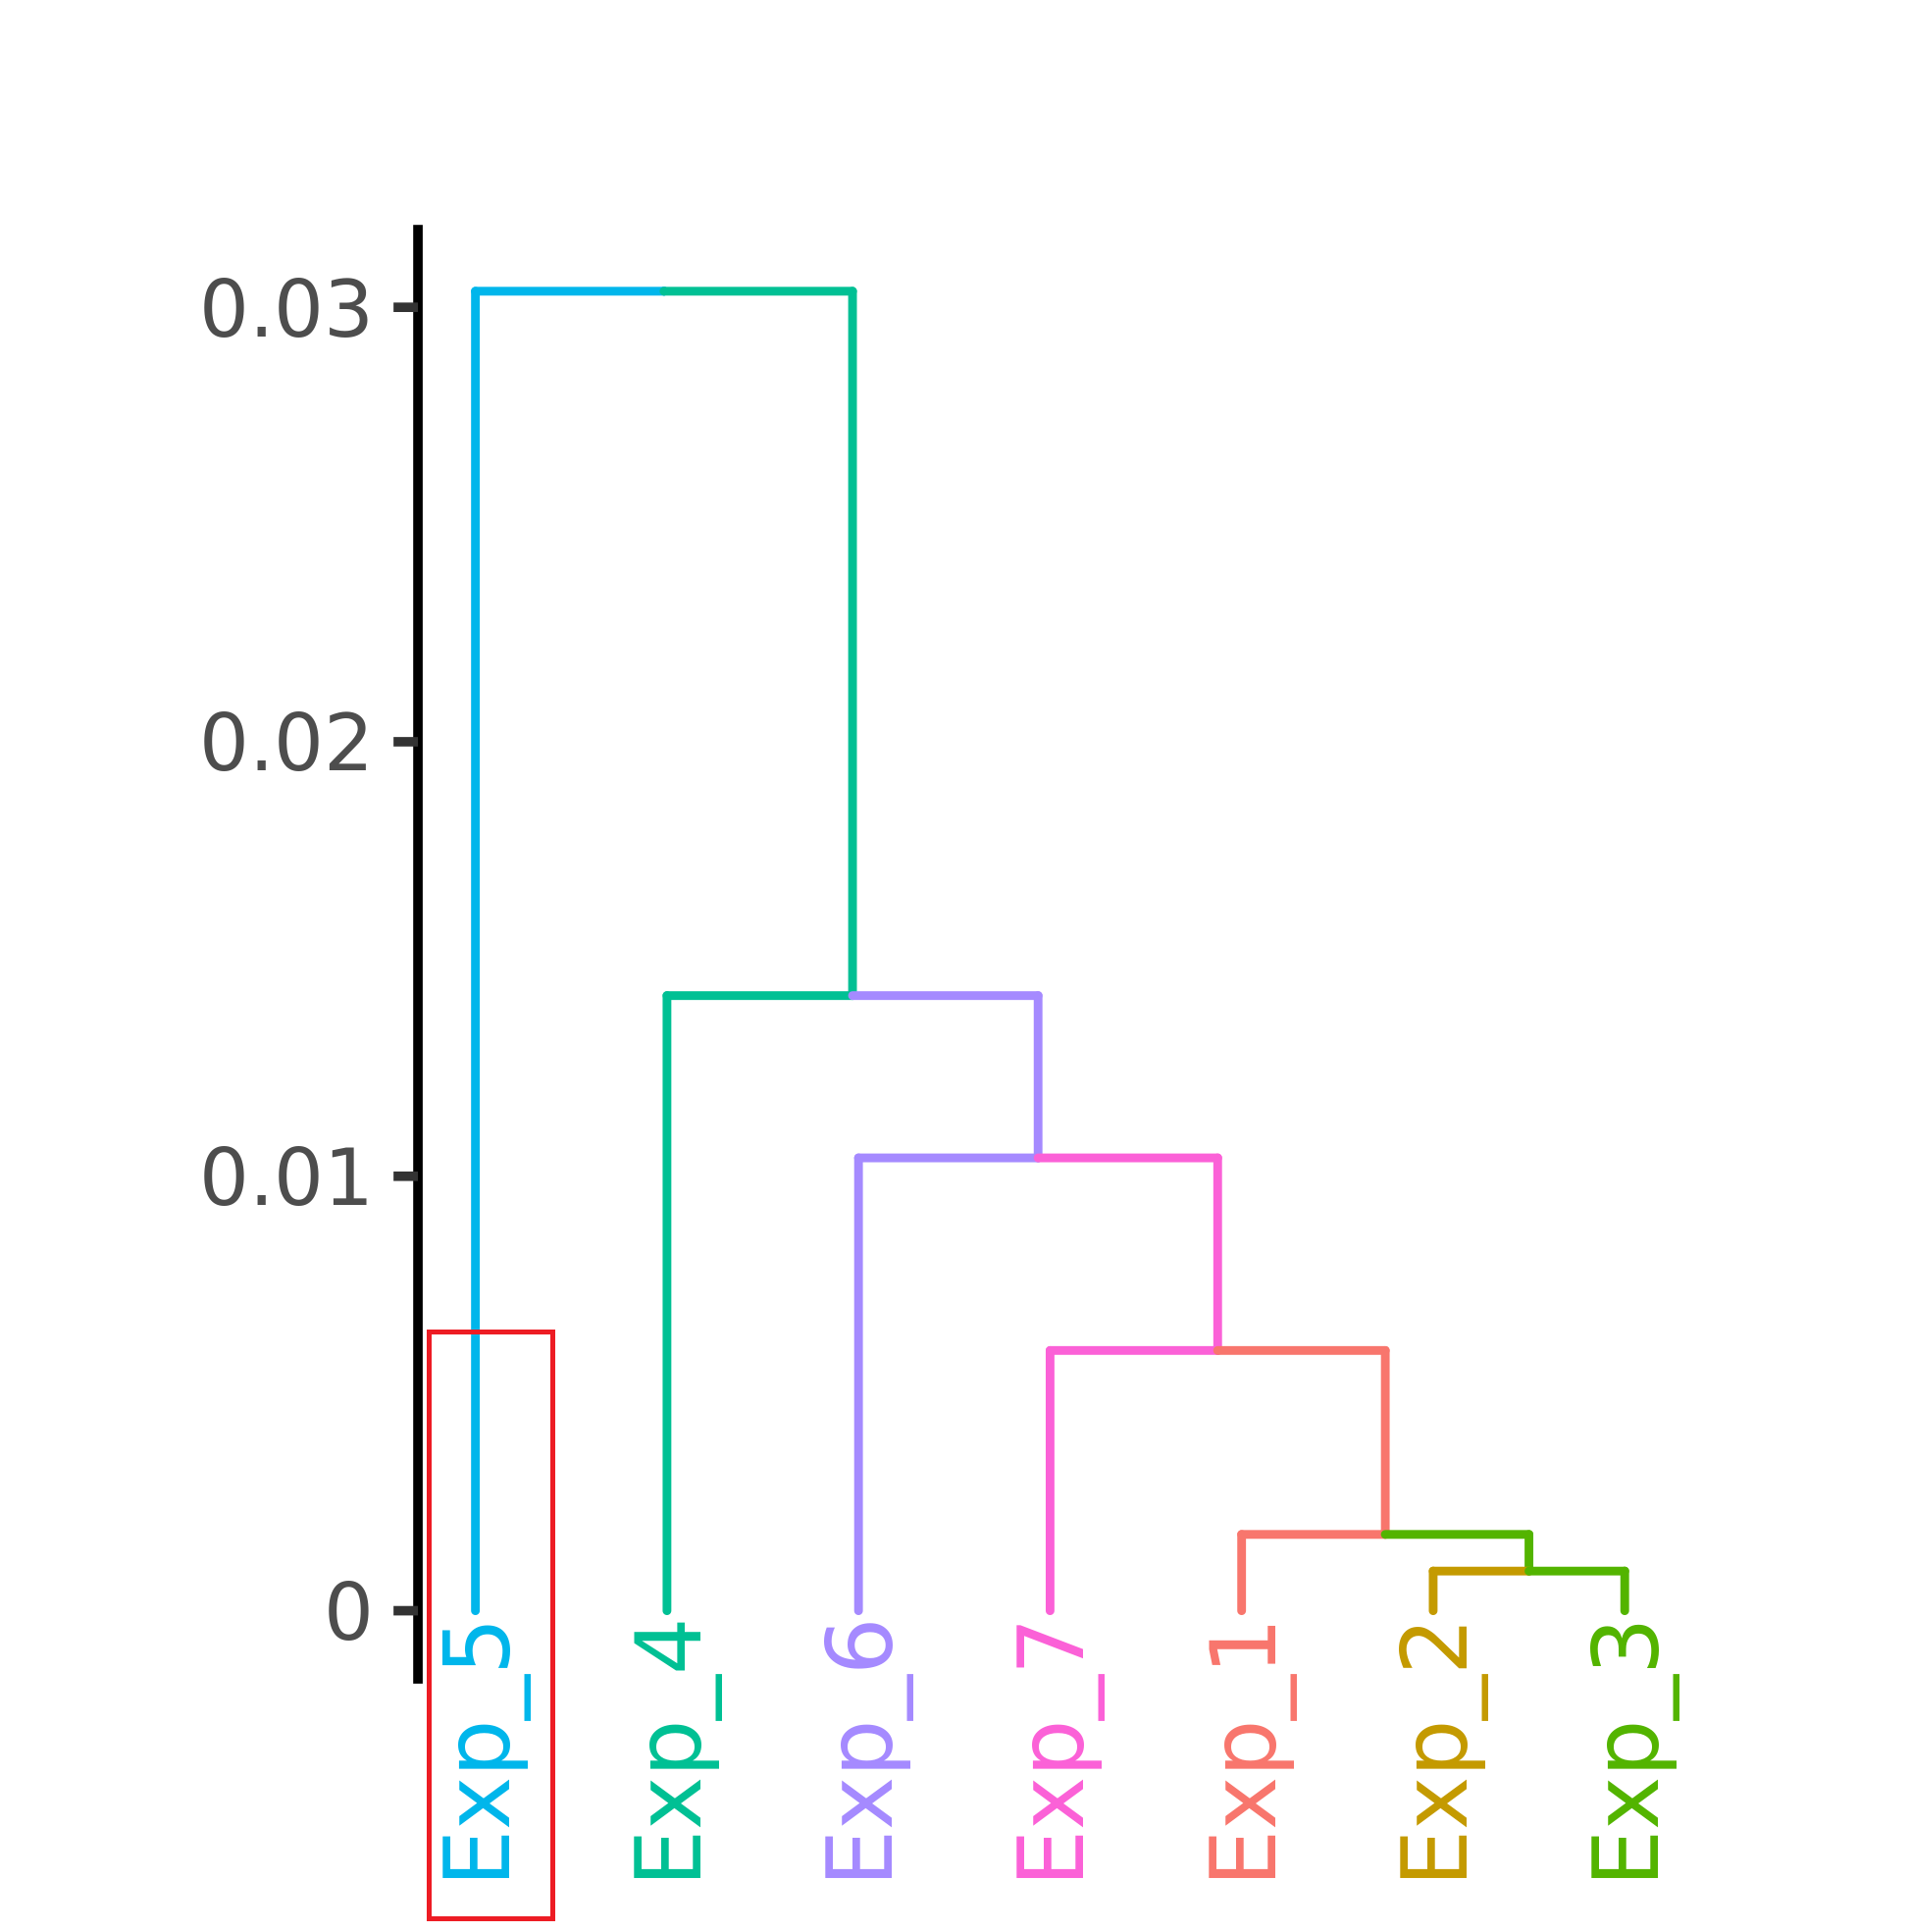
\includegraphics[width=0.5\textwidth]{fst_plot}
    \caption{$F_{st}$ statistic calculated between population groups indicate genetic divergence between the groups. The dendrogram was constructed by applying multidimensional scaling on pairwise $F_{st}$ matrix to show clustering between recently developed (outlined by the red box) and PGR derived population groups.}
    \label{fig_fst_plot}
\end{figure}

\textit{The environment relationship matrix reveals no environment relationship structure}

The ERM was utilized to examine the presence of environmental clusters, but the analysis did not uncover any discernible pattern. This finding can be interpreted in two ways: 1. There are no environmental clusters present in the tested environments, or 2. There was an error in the calculation of the ERM. The latter possibility could be attributed to either poor-quality input data or an incorrect calculation method. However, since the data is sourced from a reliable pipeline, its quality is assured. To further investigate the calculation method, the ERM was computed using intervals of 5 and 10 days, in addition to the original 30-day interval. The null hypothesis, suggesting no relationship between ECs derived from the 5, 10, and 30-day intervals, was rejected based on the results of the mantel.test() function in R (Paradis and Schliep, 2019). Consequently, it was concluded that the examined environments lack any underlying structure and are truly diverse. Studies have demonstrated that environment relationship matrix can be used to derive an approximated GxE matrix \cite{de2020data}, but the same was not a part of curent study. 

\textit{Dynamic CNN outperforms E-GBLUP for predicting average line grain yield} 

The performance of E-GBLUP and dynamic CNN models was benchmarked using three cross-validation scenarios. In the first scenario, traditional cross-validation was employed, where genotypes were randomly divided into a training and a test population in an 80:20 ratio. CNN model outperformed E-GBLUP for predicting line grain yield (Fig. \ref{fig_pred_corr_res_NN_2}). For the second scenario, stratified cross-validation was implemented to account for genetic distinctness observed in one experimental series (Fig. \ref{fig_pred_corr_res_NN_2}). The results showed slightly higher prediction accuracy in some cases compared to traditional cross-validation, but the overall trend of higher performance in case of lines was preserved here. Overall, Convolutional Neural Networks (CNN) exhibited superior performance compared to the traditional GBLUP based method, especially when dealing with extensive data or when flexibility in the genetic structure of training and test populations was required.

\begin{figure}[h]
    \centering
    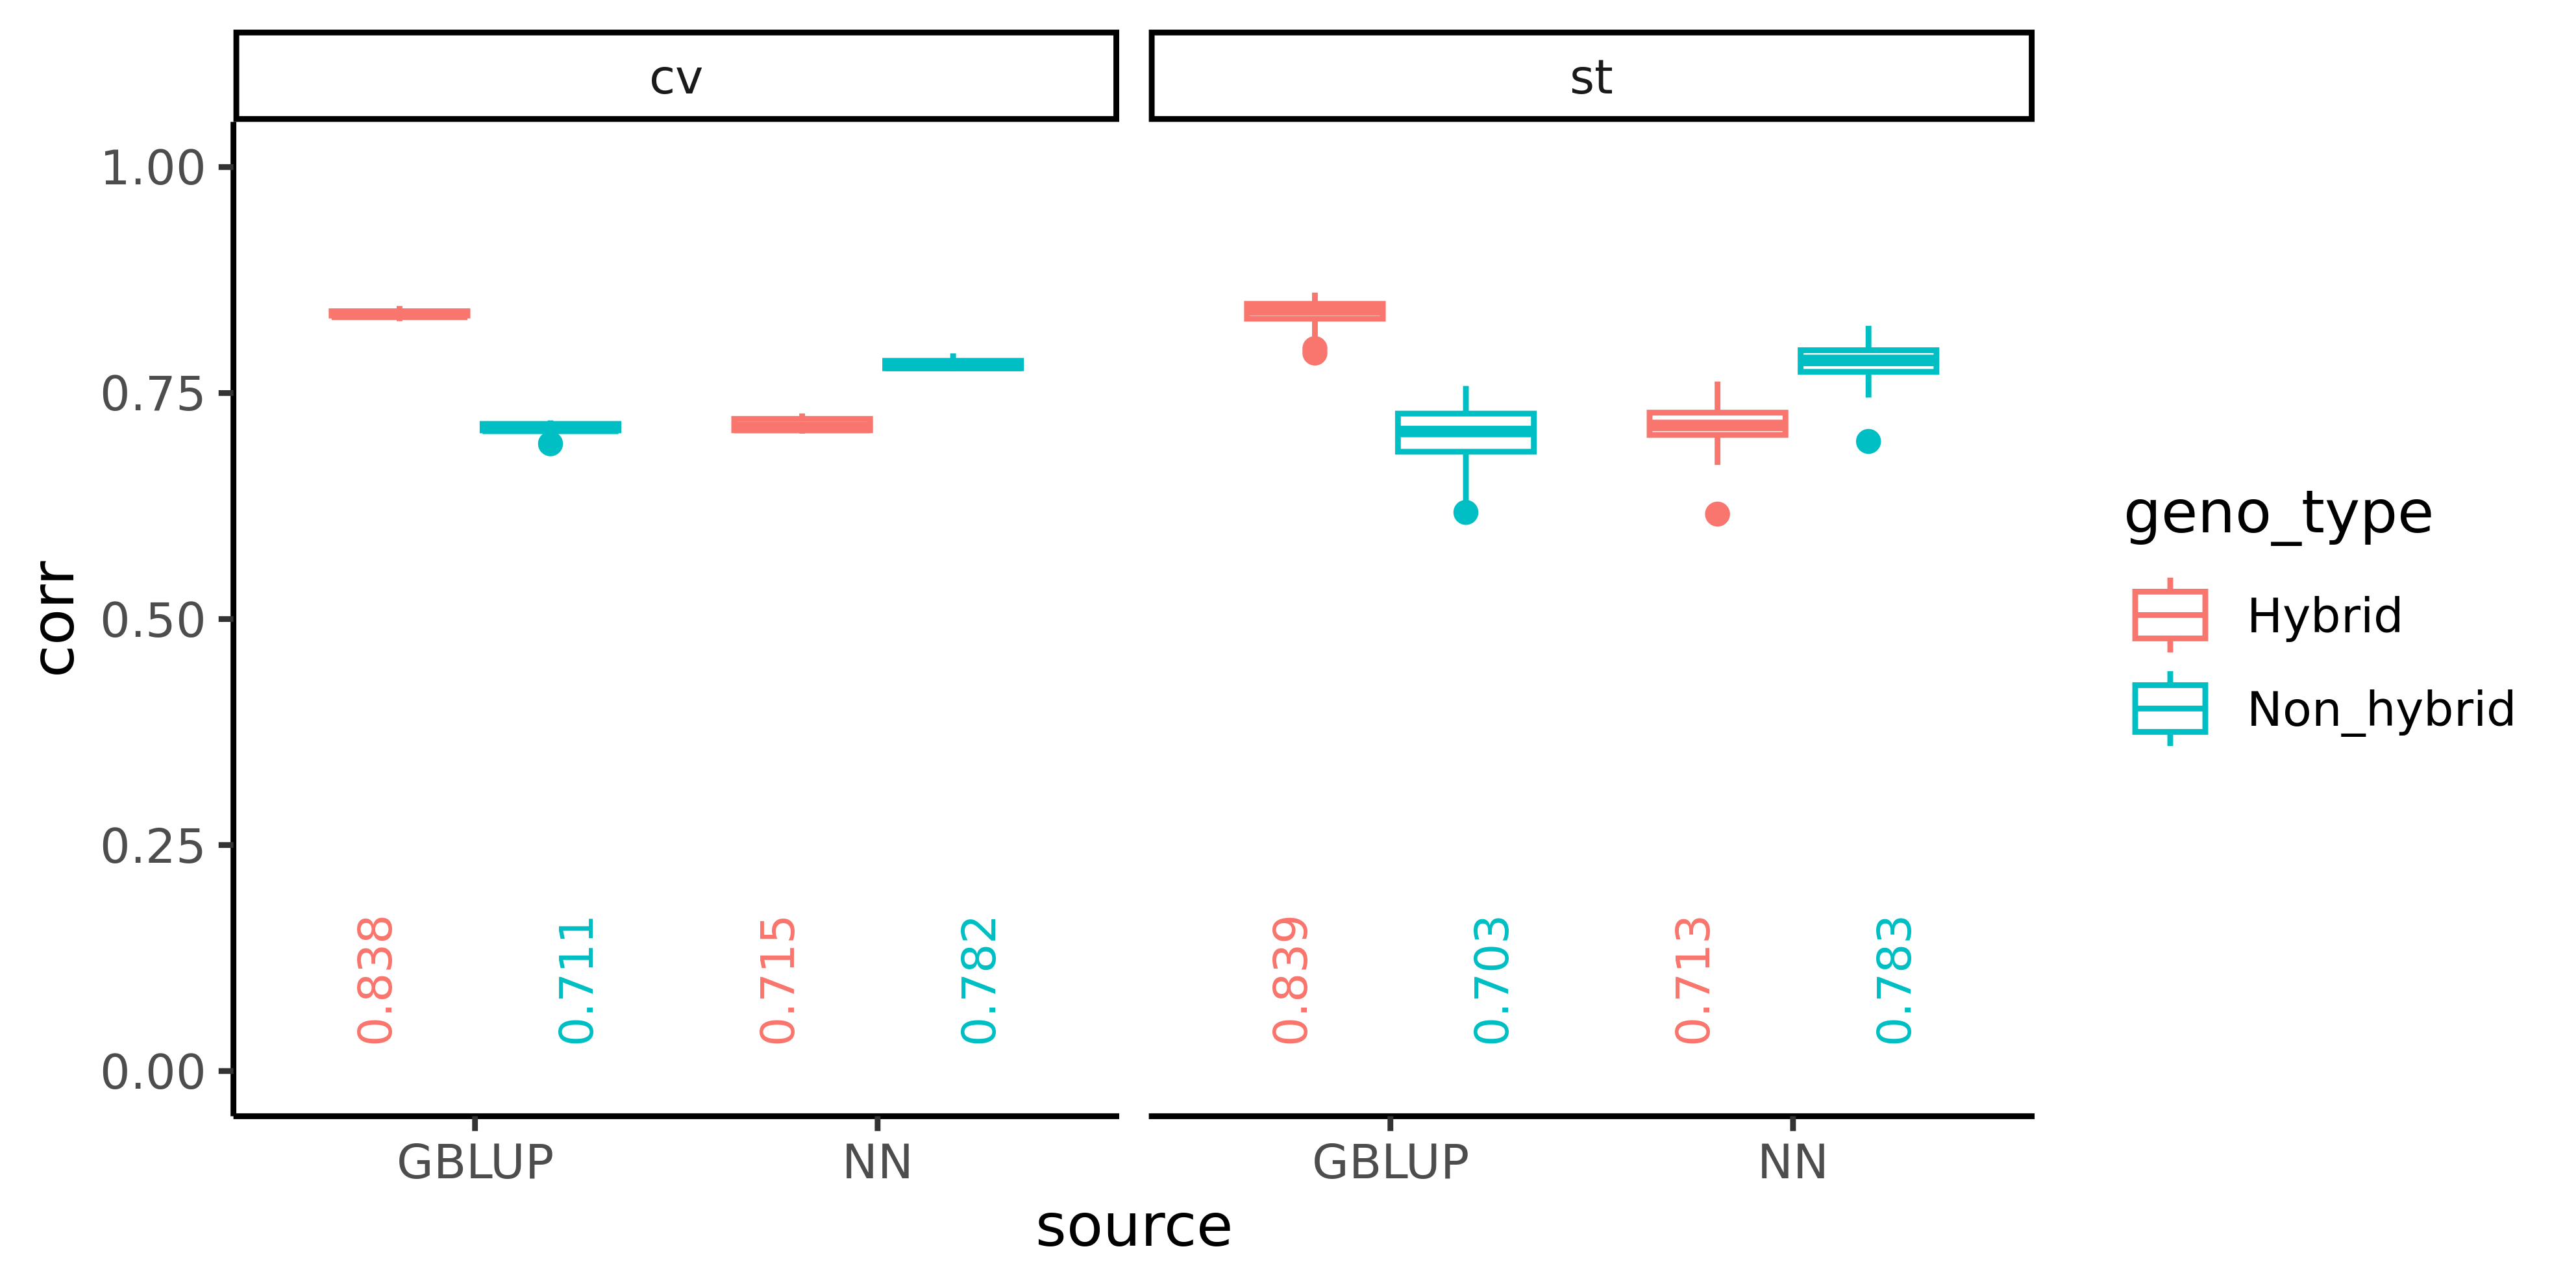
\includegraphics[width=0.9\textwidth]{pred_corr_res_NN_2}
    \caption{Genomic prediction accuracy (corr on y-axis between 0 to 1 ) of GBLUP and Convolutional Neural Networks (NN) for mean grain yield across sites under 5-fold cross validation (cv) and stratified cross validation (st). Results are shown separately for hybrids and lines.}
    \label{fig_pred_corr_res_NN_2}
\end{figure}

\section{Conclusions}

"ToDo ToDo ToDo ToDo ToDo ToDo ToDo ToDo ToDo ToDo ToDo ToDo ToDo ToDo ToDo ToDo ToDo ToDo ToDo ToDo ToDo ToDo ToDo ToDo ToDo ToDo ToDo ToDo ToDo ToDo ToDo ToDo ToDo ToDo ToDo ToDo ToDo ToDo ToDo ToDo ToDo ToDo ToDo ToDo ToDo ToDo ToDo ToDo ToDo ToDo ToDo ToDo ToDo ToDo ToDo ToDo ToDo ToDo ToDo ToDo ToDo ToDo ToDo ToDo ToDo ToDo ToDo ToDo ToDo ToDo ToDo ToDo ToDo ToDo ToDo ToDo ToDo ToDo ToDo ToDo ToDo ToDo ToDo ToDo ToDo ToDo ToDo ToDo 120 words ToDo ToDo ToDo ToDo ToDo ToDo ToDo ToDo ToDo ToDo ToDo ToDo ToDo ToDo ToDo ToDo ToDo ToDo ToDo ToDo ToDo ToDo ToDo ToDo ToDo ToDo ToDo ToDo ToDo ToDo ToDo ToDo ToDo ToDo ToDo ToDo ToDo ToDo ToDo ToDo ToDo ToDo ToDo ToDo ToDo ToDo ToDo ToDo ToDo ToDo ToDo ToDo ToDo ToDo ToDo ToDo ToDo ToDo ToDo ToDo ToDo ToDo ToDo ToDo ToDo ToDo"

\printbibliography%if you use biblatex/Biber
\end{document}